\documentclass[11pt]{article}

%% MinionPro fonts 
%\usepackage[lf]{MinionPro}
%\usepackage{MnSymbol}
\usepackage{microtype}

%% Margins
\usepackage{geometry}
\geometry{verbose,letterpaper,tmargin=1in,bmargin=1in,lmargin=1in,rmargin=1in}

%% Other packages
\usepackage{amsmath}
\usepackage{amsfonts}
\usepackage{amsthm}
\usepackage[shortlabels]{enumitem}
\usepackage{titlesec}
\usepackage{soul}
\usepackage{tikz}
\usepackage{mathtools}
\usepackage{pgfplots}
\usepackage{tikz-3dplot}
\usepackage{algorithmic}
\usepackage[export]{adjustbox}
\usepackage{tcolorbox}
\usepackage{mathrsfs}
\usepackage{multicol}
\usepackage{framed}
\usepackage{optprog}

%% Paragraph style settings
\setlength{\parskip}{\medskipamount}
\setlength{\parindent}{0pt}

%% Change itemize bullets
\renewcommand{\labelitemi}{$\bullet$}
\renewcommand{\labelitemii}{$\circ$}
\renewcommand{\labelitemiii}{$\diamond$}
\renewcommand{\labelitemiv}{$\cdot$}

%% Colors
\definecolor{rred}{RGB}{204,0,0}
\definecolor{ggreen}{RGB}{0,145,0}
\definecolor{yyellow}{RGB}{255,185,0}
\definecolor{bblue}{rgb}{0.2,0.2,0.7}
\definecolor{ggray}{RGB}{190,190,190}
\definecolor{ppurple}{RGB}{160,32,240}
\definecolor{oorange}{RGB}{255,165,0}

%% Shrink section fonts
\titleformat*{\section}{\normalsize\bf}
\titleformat*{\subsection}{\normalsize\bf}
\titleformat*{\subsubsection}{\normalsize\it}

% %% Compress the spacing around section titles
\titlespacing*{\section}{0pt}{1.5ex}{0.75ex}
\titlespacing*{\subsection}{0pt}{1ex}{0.5ex}
\titlespacing*{\subsubsection}{0pt}{1ex}{0.5ex}

%% amsthm settings
\theoremstyle{definition}
\newtheorem{problem}{Problem}
\newtheorem{example}{Example}
\newtheorem*{theorem}{Theorem}
\newtheorem*{bigthm}{Big Theorem}
\newtheorem*{biggerthm}{Bigger Theorem}
\newtheorem*{bigcor1}{Big Corollary 1}
\newtheorem*{bigcor2}{Big Corollary 2}

%% tikz settings
\usetikzlibrary{calc}
\usetikzlibrary{patterns}
\usetikzlibrary{decorations}
\usepgfplotslibrary{polar}

%% algorithmic setup
\algsetup{linenodelimiter=}
\renewcommand{\algorithmiccomment}[1]{\quad// #1}
\renewcommand{\algorithmicrequire}{\emph{Input:}}
\renewcommand{\algorithmicensure}{\emph{Output:}}

%% Answer box macros
%% \answerbox{alignment}{width}{height}
\newcommand{\answerbox}[3]{%
  \fbox{%
    \begin{minipage}[#1]{#2}
      \hfill\vspace{#3}
    \end{minipage}
  }
}

%% \answerboxfull{alignment}{height}
\newcommand{\answerboxfull}[2]{%
  \answerbox{#1}{6.38in}{#2} 
}

%% \answerboxone{alignment}{height} -- for first-level bullet
\newcommand{\answerboxone}[2]{%
  \answerbox{#1}{6.0in}{#2} 
}

%% \answerboxtwo{alignment}{height} -- for second-level bullet
\newcommand{\answerboxtwo}[2]{%
  \answerbox{#1}{5.8in}{#2}
}

%% special boxes
\newcommand{\wordbox}{\answerbox{c}{1.2in}{.7cm}}
\newcommand{\catbox}{\answerbox{c}{.5in}{.7cm}}
\newcommand{\letterbox}{\answerbox{c}{.7cm}{.7cm}}

%% Miscellaneous macros
\newcommand{\tstack}[1]{\begin{multlined}[t] #1 \end{multlined}}
\newcommand{\cstack}[1]{\begin{multlined}[c] #1 \end{multlined}}
\newcommand{\ccite}[1]{\only<presentation>{{\scriptsize\color{gray} #1}}\only<article>{{\small [#1]}}}
\newcommand{\grad}{\nabla}
\newcommand{\ra}{\ensuremath{\rightarrow}~}
\newcommand{\maximize}{\text{maximize}}
\newcommand{\minimize}{\text{minimize}}
\newcommand{\subjectto}{\text{subject to}}
\newcommand{\trans}{\mathsf{T}}
\newcommand{\bb}{\mathbf{b}}
\newcommand{\bx}{\mathbf{x}}
\newcommand{\bc}{\mathbf{c}}
\newcommand{\bd}{\mathbf{d}}

%% LP format
%    \begin{align*}
%      \maximize \quad & \mathbf{c}^{\trans} \mathbf{x}\\
%      \subjectto \quad & A \mathbf{x} = \mathbf{b}\\
%                       & \mathbf{x} \ge \mathbf{0}
%    \end{align*}

%Space between rows:
%\def\arraystretch{2.2}
%
%Space between columns:
%\arraycolsep=1.4pt


%% Redefine maketitle
\makeatletter
\renewcommand{\maketitle}{
  \noindent SA405 -- AMP \hfill Rader \S 13.1  \\

  \begin{center}\Large{\textbf{\@title}}\end{center}
}
\makeatother

%% ----- Begin document ----- %%
\begin{document}
  
\title{Lesson 12.  IP Formulations Part 1}

\maketitle

%%%

\renewcommand\labelitemi{--}
\section{Solving Integer Programs can be \emph{Really} Hard!}

Suppose we are solving the following integer program:

\begin{optprog*}
max & \objective{12 x_1 + 13 x_2} \\
st  & 6 x_1 + 7 x_2 & \leq & 21 \\
    & x_1, x_2 & \in & \mathbb{Z}^+
\end{optprog*}

Usually, everyone's first thought for solving IPs is to solve the LP and then round to the nearest integer. Let's try that here:

\vfill

If we solve the LP we get the solution: \vspace{0.5cm}

Rounding this solution, we get an IP solution of: \vspace{0.5cm}

Is this the optimal solution to the IP? \vspace{1cm}

\begin{tcolorbox}
In general, IPs are \textbf{significantly harder} to solve than LPs.
\end{tcolorbox}

\begin{itemize}
\item In the next two lessons, we will discuss why IPs are harder than LPs and why the way we model IP problems can impact solver performance.
\item In lesson 14 we will learn about the \textbf{branch and bound algorithm} which is a method to solve IPs.
\end{itemize}

\newpage
\section{Review Linear Programming Solution Techniques}

\subsection{Types of LP solutions}

\textbf{Theorem:} Every LP's solution is EXACTLY one of the following:
	\begin{enumerate}
	\item Unique optimal solution
	\item Multiple optimal solutions
	\item Unbounded LP
	\item Infeasible LP
	\end{enumerate}

\begin{problem}
Sketch graphs which illustrate each of the types of LP solutions.
\end{problem}

\vfill

\begin{tcolorbox}
These types of solutions are also true for integer programs. Recall that if an LP has an optimal solution, it always occurs at a corner point.
\end{tcolorbox}

\newpage

\section{Integer Program Formulations}

\begin{tcolorbox}
A \textbf{formulation} of an integer (linear) program is a set of linear \wordbox that capture ALL of the \wordbox integer points, and NO OTHER integer points.
\end{tcolorbox}

\vfill

\begin{tcolorbox}
The \textbf{LP relaxation} of an IP is the LP that is formed by relaxing (i.e., removing) the integer requirement on the variables.
\end{tcolorbox}

\begin{problem}  
Below are two integer programs, along with the diagrams of their constraints.

\begin{multicols}{2}

{\bf Integer Program A}
\begin{align*}
      \maximize \quad & 8x + 7y \\
      \subjectto \quad & -18x + 38y ~~\leq~~ 133\\
                       & 13x + 11y ~\leq~ 125\\
                       & 10x - 8y ~\leq~ 55\\
                       & x,~y ~\geq~ 0, \text{ integer}
\end{align*}
\vspace{6cm}

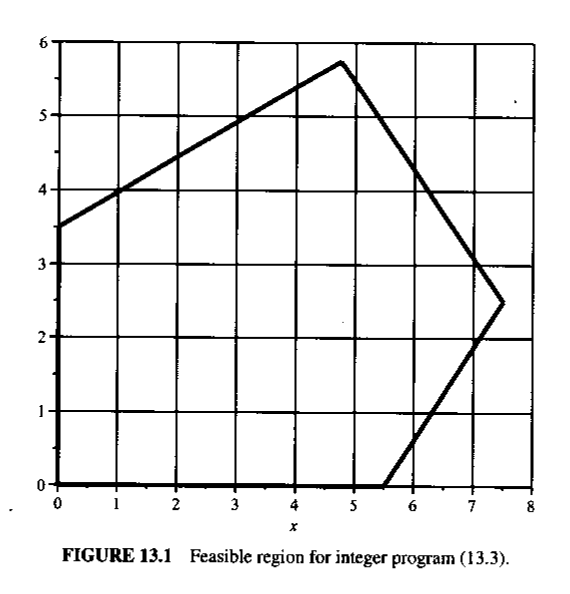
\includegraphics[width = 0.4\textwidth]{formulation_bad}
\end{multicols}

\begin{multicols}{2}

{\bf Integer Program B}
\begin{align*}
      \maximize \quad & 8x + 7y \\
      \subjectto \quad & -x+2y ~\leq~ 6\\
                       & x + y ~\leq~ 10\\
                       & x - y ~\leq~ 5\\
                       & x ~\leq~ 7\\
                       & y ~\leq~ 5\\
                       & x,~y ~\geq~ 0, \text{ integer}
\end{align*}
\vspace{6cm}

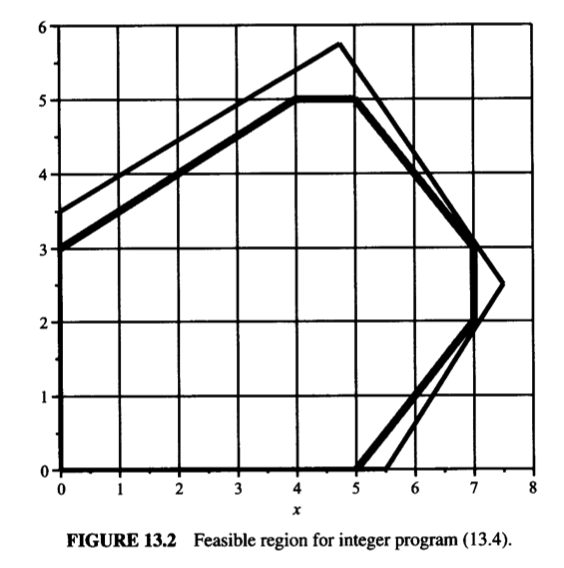
\includegraphics[width = 0.4\textwidth]{formulation_ideal}
\end{multicols}

\newpage

\begin{enumerate}[(a)]
   \item On the diagrams, identify all feasible solutions to both IPs. \vfill
   \item Are the integer feasible regions for IP A and IP B different or the same? \vfill
   \item Are the feasible regions of the LP relaxations of IP A and IP B different or the same? \vfill
   \item What does this mean about problems A and B? \vfill
   \item Based on these graphs, will the optimal solution of an IP always occur at a corner point? \vfill
   \item Which of these formulations is easier to solve? Why? \vfill

\end{enumerate}
\end{problem}

\newpage

\subsection{Better Formulation $\Rightarrow$ Better Bound}

Now let's consider the relationship between an IP and its LP relaxation.

\bigskip

In general:
	\begin{itemize}
	\item If we are solving a \textbf{maximization} IP, the solution of its LP relaxation provides a \wordbox bound on the solution of the IP problem.
	\item If we are solving a \textbf{minimization} IP, the solution of its LP relaxation provides a \wordbox bound on the solution of the IP problem.
	\end{itemize}

The \textbf{tighter} a formulation, the \wordbox bound you obtain via the LP relaxation.

\begin{tcolorbox}
This idea is key for solving IPs!
\end{tcolorbox}	
\begin{problem}
Sketch a problem which proves if we're maximizing, $z_{LP} \geq z_{IP}$ and vice versa if minimizing.
\end{problem}
\vfill

Often the decision of how to formulate an IP comes down to a tradeoff between the formulation quality and number of constraints.
\begin{itemize}
\item More constraints can lead to a better (tighter) formulation, but: \vspace{0.5in}
\item Fewer constraints lead to a weaker formulation but: \vspace{0.5in}
\end{itemize}	





\end{document}
